\documentclass[conference]{IEEEtran}

\IEEEoverridecommandlockouts
\usepackage{cite}
\usepackage{amsmath,amssymb,amsfonts}
\usepackage{algorithmic}
\usepackage{graphicx}
\usepackage{textcomp}
\usepackage{xcolor}
\usepackage{fancyhdr}
\usepackage{booktabs}
\usepackage{siunitx}
\usepackage{lipsum}
\usepackage{graphicx}

\def\BibTeX{{\rm B\kern-.05em{\sc i\kern-.025em b}\kern-.08em
    T\kern-.1667em\lower.7ex\hbox{E}\kern-.125emX}}

\fancypagestyle{firstpagefooter}{%
  \fancyhf{}
  \renewcommand\headrulewidth{0pt}
  \fancyfoot[R]{NotebookNet: An Explorative Machine Learning Approach in Code Comprehension}
}

\pagestyle{empty}

\begin{document}
\title{NotebookNet: An Explorative Machine Learning Approach in Code Comprehension }

\author{\IEEEauthorblockN{Amir Sotoodeh}
\IEEEauthorblockA{\textit{sotoodaa@berkeley.edu}}
University of California: Berkeley
\and
\IEEEauthorblockN{Sophie Yeh}
\IEEEauthorblockA{\textit{syeh1@berkeley.edu}}
University of California: Berkeley
\and
\IEEEauthorblockN{Qian Qiao}
\IEEEauthorblockA{\textit{qianqiao@berkeley.edu}}
University of California: Berkeley}

\maketitle

\thispagestyle{firstpagefooter}

\begin{abstract}
Research teams across the world are interested in exploring the domain of assistive technology for software engineers. Much like Github Copilot and Amazon CodeWhisperer, understanding natural language and its intrinsic relationship with programming languages could lead to significant improvements in developer productivity and revolutionize the industry standard for writing code. Our project aims to predict the order of markdown code cells based on python code cells in Jupyter Notebooks using the AI4Code Kaggle dataset published by Google. The main evaluation metric is Kendall’s tau, which is frequently the metric of choice for text ranking and specifically the AI4 Code competition. Our highest performing model uses CodeBert and Bert tokenizers with a linear layer and single feature engineering tensor which achieved a Kendall’s tau of 0.79 with room for additional tuning.
\end{abstract}

\begin{IEEEkeywords}
machine learning, natural language processing, bert, embeddings
\end{IEEEkeywords}



\section{Introduction}
Recently, self-attention based deep learning architectures have outperformed conventional recurrent and LSTM neural networks in natural language processing tasks. Given that RNNs stuffer from vanishing gradient issues and LSTM networks tend to overfit, our approach leans towards transformers to learn contextual and semantic meaning between code and markdown (Yu et al. 2021).

Given an understanding of code cell relationships to markdown comments, it is possible to develop productivity tools that aid in the automatic reconstruction of a notebook's order and readability. With the Google AI4Code Kaggle competition and the rising popularity of transformer neural network architectures, we aim to explore the performance of attention within a ranking setting to predict the correct ordering of the cells in a given Jupyter notebook whose markdown cells have been shuffled.

Several challenges we addressed were the size of the data, effect of performance due to different languages in the dataset, and text normalization. In the process, we utilized SpaCy models to classify the notebooks by language and performed various experiments with frozen/unfrozen Bert models, code cell embeddings, and pooling techniques.


\section{Literature Review}
Although our project has a novel research objective of ordering shuffled markdown cells to match python code cells, it is fundamentally a ranking task with many existing research findings in recent years. Text ordering was originally a task to test a machine’s understanding of entities, events and relationships using nearby sentences in a text corpus (Chowdhury et al. 2021). Early methods to solve this problem involve using different categories of features like coherence clues, entity grids, named-entity categories, and syntactic features. More recent works use deep learning methods such as pointer networks, topological sorting, and, the most promising, BERT encoders to score sentences and produce a rank.

In April 2020, Kumar et al. was the first to approach text ordering as a ranking problem with RankTxNet. Using a BERT sentence encoder, randomly initialized Transformer paragraph encoder, and a feed-forward neural network decoder, a relevance score for each sentence was calculated to produce the ranking. The paper also explored three popular ranking loss functions: pointwise ranking loss, pairwise ranking loss, and listwise ranking loss. Pointwise ranking loss is a regression approach where each sentence is mapped to a score between 0 and 1. Pairwise ranking loss computes the margin ranking loss between pairs of sentences. Lastly, listwise ranking loss calculates the probability of a sentence being on top. Their results demonstrated that pairwise and listwise methods outperformed pointwise methods across the board and ListMLE performed the best in most cases. In response to Kumar et al.’s findings, the research direction focused on leveraging BERT in novel ways to improve performance. A few months after Kumar’s publication, BERT-enhanced Relational Sentence Ordering Network (BERSON) was introduced as a BERT-based model that constructs a pairwise relationship representation for each sentence pair (Cui et al. 2020), outperforming RankTxNet. Reorder-BART (RE-BART) uses BART to encode the entire shuffled sequence of text rather than pointwise and pairwise to capture the interactions between all sentences (Chowdhury et al. 2021). This out-performed BERSON by a small margin.

Within text-ordering research, Kendall’s Tau was the most widely-used metric. Kendall’s tau, proposed in 2003, is “a measure of rank correlation” that “estimat[es] the distance between a system-generated and a human-generated gold-standard order (Lapata 2006). Although less widely used than Spearman’s rank correlation coefficient in the NLP field as a whole, Kendall’s tau is the metric of choice in text-ordering tasks due to its correlation with human judgment. While prior text ordering research are primarily language-based models, our project required research into encoding python code and CodeBERT was the first and most noteworthy bimodal model developed by Microsoft pre-trained for natural language code search and code documentation (Feng et al. 2020). Published in 2020, it has opened the doors to new research on processing code-based text. Thus, our research question bridges the gap between CodeBERT’s gateway into code processing, code translation, and text translation.

\section{Dataset}
The primary and sole dataset of choice from a Kaggle competition which comprises about 160,000 Jupyter notebooks. The notebooks of the dataset have its contents stored as JSON files and a central excel spreadsheet containing the correct orders of each cell of a notebook as a list of unique cell identifiers. This required a merging of the various data components to achieve a suitable dataset in preparation for training. Each individual cell is classified as code or markdown, which contains unprocessed free-text with an ensemble of unicode characters. The test and validation set provided by the competition contains ordered python code cells with shuffled markdown cells, in which the goal of the model is to determine the correct order of markdown cells relative to the code cells.

\subsection{English Notebooks}
Given that natural language processing has a large emphasis on semantic meaning and order between sequences of characters, we aim to explore the variability and generalizability of our model’s performance on various languages. However, for simplicity, we opted to focus a large portion of experiments on English only notebooks to avoid unwanted biases from the severe class imbalance discussed below.

\begin{figure}[h]
  \centering
  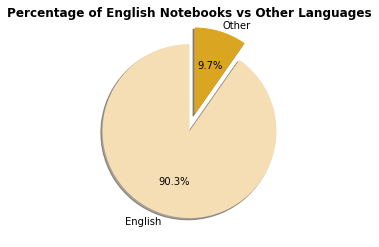
\includegraphics[width=\linewidth]{eng_percent}
  \caption{Pie chart representing the prominence of English notebooks in the dataset.}
\end{figure}

\begin{figure}[h]
  \centering
  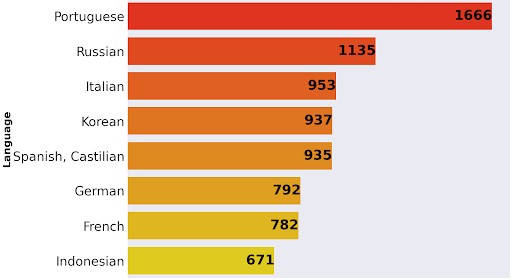
\includegraphics[width=\linewidth]{freq}
  \caption{Bar chart of the top 8 non-english notebooks in the dataset. There are roughly 16,000 english notebooks, indicating a severe language imbalance.}
\end{figure}

%% TODO: ADD REFERENCE TO SPACY HERE
In order to classify the dataset based on the language embedding in the markdown we utilized SpaCy models. The SpaCy model En\_core\_web\_sm, which is a pipeline trained on written web text, allowed us to utilize state-of-the-art (SOTA)  (92.0\% parser, 97.48\% tagger, 85.5\% accuracies named entity recognition(NER)) natural language models to classify languages of the  notebooks with ease.  By simply extracting the Markdown cells in each notebook, SpaCy returns the language of the string with the corresponding probability.


After ingesting the entire dataset of notebooks, we concluded that there are roughly 44 distinct languages in the whole train dataset, 90.3\% of notebooks are in English and 9.7\% are in other languages, like 'Portuguese', 'Russian', 'Turkish', 'Japanese', 'Italian', 'Korean', 'Spanish, Castilian', 'German', 'French', 'Indonesian', 'Catalan, Valencian', 'Vietnamese', 'Tagalog’ and so on.


\subsection{Text Normalization}
%% TODO: ADD INFOGRAPHIC SHOWING SOME TEXT NORMALIZATION?
Markdown and code content are inherently noisy given the vast set of characters and varying syntactic styles that can be unique based on an individual’s preference. Additionally, the markdown language contains a distinct set of characters that are used to enhance or modify the appearance of the rendered content, which may or may not have a significant effect on the positioning of the cell.  With this in mind, several text normalization strategies were applied, which include and are not limited to: markdown special character removal, lowercasing, lemmatization, underscore conversion to space, multiple space removal, and HTML tag removal. Different variations and combinations of such normalizations were applied, in which we found that applying all forms of normalization of text improved the overall performance of each of the models. Thus each of the reported results were results post-normalization of the text in the dataset.

\subsection{Cell Ranking}
Each notebook has all the code cells followed by the markdown cells. In the training dataset, the code cells are in the correct relative order, while the markdown cells are shuffled. We determine the correct rank of the cells within a notebook by referencing the true ordering of cells and computing the percentile rank. Given the relative ordering of the code cells among themselves, we will use a transformer-based model to predict where the markdown cells should be placed among the code cells within a notebook. Within the training set, given the correct order of all cells, a row-wise percentile rank is calculated, which yields a floating point value [0, 1] for each row.

%% This is placed above to ensure it ends up at the top of the page.
\begin{figure*}
  \centering
  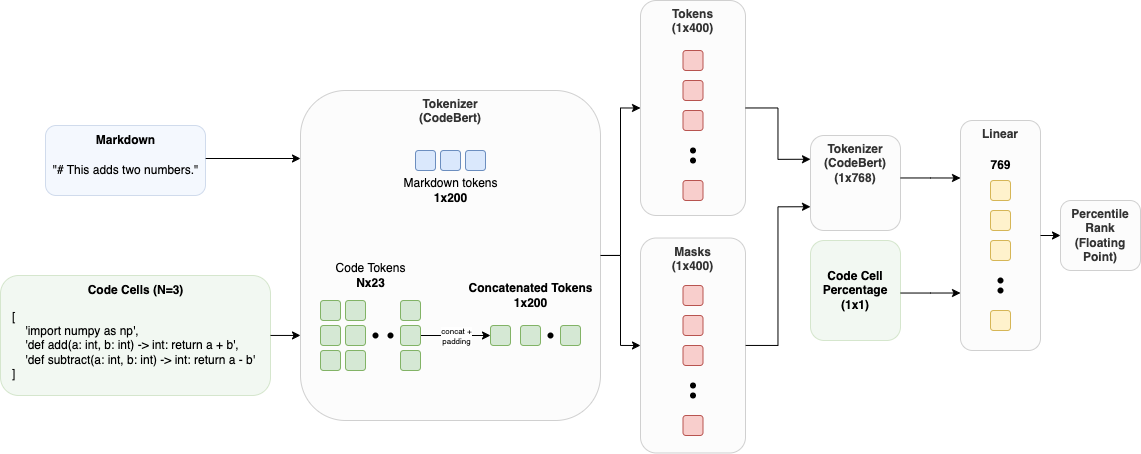
\includegraphics[width=\textwidth]{baseline}
  \caption{The NotebookNet point-wise approach. Input are code cells, a markdown cell, and a feature engineered code cell percentage tensor. Output is a percentile rank floating point tensor.}
\end{figure*}

\subsection{Feature Engineering}
As part of experimentation, the notebooks as a whole have specific metadata and characteristics that could be feature engineered into the models. Namely, the number of code cells, the number of markdown cells, and the total number of cells may or may not have a significant impact on the regression output score of a point-wise approach. With this in mind, various combinations of feature engineering tensors were included within model iteration and were included or removed based on performance indicators.

\subsection{Tokenization}
Various tokenization strategies were applied depending on the model in question. Primarily, a CodeBert tokenizer was applied in the baseline model, whereas a CodeBert and BertBaseUncased tokenizer were applied in the subsequent models. To keep the experiment variation minimal, the lengths of the produced tokens and masks were limited to 400. This 400 is split into 200 tokens for code and 200 tokens for markdown. Given that the input to the model will contain one markdown cell, and several code cells, each individual code cell is tokenized in batches of length 23, and concatenated/flattened up to a length of 200 (see figure below in methods). These 400 tokens are then fed into the CodeBert or Bert models with pre-trained self-attention mechanisms on code-specific tasks.

\section{Methods}

Given that Codebert was trained for general-purpose NLP tasks such as natural language codesearch, and code documentation generation, we chose to explore this transformer based architecture as the backbone. Subsequent models explore the addition of a vanilla Bert Base Uncased tokenizer and model.

For each model, we obtain the embedding token matrix $A \in \mathbb{R}^{d \times N}$, where $d$ is the embedding dimension and $N$ is the number of tokens. All variants of NotebookNet were trained on a g4dn.4xlarge EC2 instance, which allowed 4 concurrent training jobs to utilize the GPU fully. As discussed previously, for consistency, code tokens are of length 200, markdown tokens are of length 200 for a total output size of $N \times 400$. The formulation, in general, for each of the models is roughly a variant of the following:

\begin{figure}[h]
  \centering
  \[ X_{out} = Linear(T_{codebert}(X_{input})) \]
  \caption{T = transformer attention blocks, Input = tokenized cells}
\end{figure}

All variants of the models are optimized by minimizing L1 Loss, or Mean Absolute Error.

\begin{figure}[h]
  \centering
  \[ L=\sum_{i=1}^{D}|x_i-y_i| \]
  \caption{MAE or L1 Loss}
\end{figure}

%% Maybe add more info + another citation here??

The core backbone of the models are optimized on the information prioritization nature of transformers, otherwise known as Attention.

\begin{figure}[h]
  \centering
  \[ Attention(Q, K, V) = softmax(\frac{QK^T}{\sqrt{d_k}})V \]
  \caption{Attention mechanism from \it{Attention Is All You Need}}
\end{figure}


\begin{figure*}
  \centering
  \includegraphics[width=\textwidth]{codebert}
  \caption{The NotebookNetV2 point-wise approach. Inputs are the same as the baseline, with the introduction of Bert Base Uncased tokenizer and model to create markdown embeddings.}
\end{figure*}

\begin{table*}[!htp]
\centering

\sisetup{detect-all}
\NewDocumentCommand{\B}{}{\fontseries{b}\selectfont}

\begin{tabular}{
  @{}
  l
  S[table-format=2.5]
  S[table-format=2.5]
  S[table-format=2.5]
  S[table-format=2.5]
  S[table-format=2.5]
  S[table-format=2.5]
  S[table-format=2.5]
  S[table-format=2.5]
  @{}
}
\toprule
Block & \multicolumn{8}{c}{Models} \\
\cmidrule(l){2-9}
& \multicolumn{2}{c}{NotebookNet} & \multicolumn{2}{c}{NotebookNet AvgPool} & \multicolumn{2}{c}{NotebookNetV2} & \multicolumn{2}{c}{NotebookNetV2-2} \\
\cmidrule(lr){2-3} \cmidrule(lr){4-5} \cmidrule(l){6-7} \cmidrule(l){8-9}
& {Size} & {Arch} & {Size} & {Arch} & {Size} & {Arch} \\
\midrule
Input &  {1x400} & {/} & {1x400} & {/} & {1x400} & {/} & {1x400} & {/} \\
CodeBert/GraphCodeBert &  {1x768} & {Transformer} & {1x768} & {Transformer} & {1x768} & {Transformer} & {1x768} & {Transformer}\\
BertBaseUncased & {/} & {Transformer} & {1x768} & {Transformer} & {1x768} & {Transformer} & {1x768} & {Transformer} \\
AvgPool1D & {/} & {/} & {(2, 0, 0) (K, S, P)} & {Pooling} & {/} & {Pooling} & {/} & {Pooling} \\
Linear & {769x1} & {MLP} & {769x1} & {MLP} & {1536x1} & {MLP} & {1536x768} & {MLP} \\
Linear & {/} & {MLP} & {/} & {MLP} & {/} & {MLP} & {768x1} & {MLP} \\
\bottomrule
\\
\end{tabular}

\caption{Model Architectures, Blocks, and Parameter sizes}

\end{table*}

\subsection{NotebookNet (Baseline)}

The baseline model (fig. 3) employs CodeBert as its primary tokenizer and backbone model followed by a linear layer inclusive of embeddings and a single feature engineering tensor (markdown cell percentage). Multiple code cells are tokenized into individual lengths of $N = 23$, which is then converted to a $1 \times 200$ feature vector (padding applied for small code cell inputs). Tokenized inputs and masks are input to a CodeBert model which outputs a $1 \times 768$ embedding vector, which regresses to a floating point percentile rank. A second variation (Baseline AvgPool1D) of the NotebookNet baseline applies an AvgPool1D layer of which the results are discussed below.

\subsection{NotebookNetV2}

\subsubsection{NotebookNetV2}
Similar to the baseline approach, CodeBert is utilized as the primary tokenizer of code cells. However, this approach differs in utilizing a vanilla BERT-based-uncased tokenizer and model for Markdown content and embedding. The embeddings of the two transformer networks are then concatenated and fed into a 1536-d linear layer with the same regressed output tensor. The second variant of this network adds an additional intermediary linear layer of size 1536x768.

\begin{figure}[h]
  \centering
  \begin{flalign}
  E &= T_{codebert}(X_{code}) + T_{bert}(X_{markdown})\\
  X_{1} &= Linear_{1536x1}(E)\\
  X_{2} &= Linear_{768x1}(Linear_{1536x768}(E))
  \end{flalign}
  \caption{E = concatenated embedding of CodeBERT and BERT-base-uncased, Eq 2 is the first variant with a single linear layer, eq 3 is the second variant with intermediary 1536x768 linear layer.}
\end{figure}

\subsubsection{GraphCodeBERT}
GraphCodeBERT is a pre-trained model for programming language, which is a multi-programming-lingual model pre-trained on NL-PL pairs in 6 programming languages (Python, Java, JavaScript, PHP, Ruby, Go). Both CodeBERT and GraphCodeBERT use a multi-layer bidirectional Transformer-based architecture. The difference between them is GraphCodeBERT considers the inherent structure of code with a dataflow graph, while CodeBERT regards a code snippet as a sequence of tokens and ignores the inherent structure of code. The GraphCodeBERT tokenizer and model was also tested, in which results are discussed in the results section below.

\begin{table}[!htp]
\centering

\sisetup{detect-all}
\NewDocumentCommand{\B}{}{\fontseries{b}\selectfont}

\begin{tabular}{
  @{}
  l
  S[table-format=3.5]
  S[table-format=3]
  S[table-format=3.2]
  S[table-format=3.2]
  @{}
}

\toprule
{Model Name} & {Runtime} & {Loss} & {\tau} \\
\midrule
{notebooknet-baseline} & {1d 12h} & 0.231 & 0.635\\
\B {notebooknet-baseline-english} & \B {1d 17h} & \B 0.1708 & \B 0.783\\
{notebooknet-baseline-pooling1d} & {1d 23h} & 0.2562 & 0.648\\
{notebooknet-v2} & {0d 16h} & 0.2225 & 0.744\\
{notebooknet-v2-english} & {2d 15h} & 0.1704 & 0.784\\
\B {notebooknet-v2-2-english} & \B {3d 2h} & \B 0.1700 & \B 0.785\\
{notebooknet-v2-frozen} & {1d 18h} & 0.0605 & 0.699\\
{notebooknet-v2-graphcodebert} & {4d 0h} & 0.4043 & 0.544\\
{notebooknet-v2-graphcodebert-english} & {3d 6h} & 0.2858 & 0.528\\
\bottomrule
\\
\end{tabular}
\caption{Results}

\end{table}

\newpage

\section{Results}

Predictions are evaluated by the Kendall tau correlation between predicted cell orders and ground truth cell orders accumulated across the entire collection of test set notebooks. The number of swaps from the predicted cell order across the entire collection of test set notebooks are summed, and similarly with the worst-case number of swaps.

\begin{figure}[h]
  \centering
  \begin{flalign}
    \tau = 1 - \frac{2S(\pi,\sigma)}{N(N-1)/2}
  \end{flalign}
  \caption{Kendall's Tau coefficient formula.}
\end{figure}

Table II compares our key experiments. The NotebookNet Baseline is trained on the entire training set including all languages and achieved a Kendall’s tau of 0.635. Adding an Average Pooling 1D hidden layer increased the score slightly to 0.648 (\textit{notebooknet-baseline-pooling1d}). When observing loss plots, it was clear that the baseline models overfit on the training data, in which adding more hidden layers improved validation metrics. Replacing CodeBert with GraphCodeBert significantly lowered the score to 0.544, which is 0.345 lower than our baseline Kendall’s Tau (\textit{notebooknet-v2-graphcodebert}). Freezing Bert layers also did not improve the model (\textit{notebooknet-v2-frozen-1lr}).

A minor ablation study was performed that suggests that there is a significant impact to the prediction score upon filtering for English only notebooks, which ultimately improved the baseline model’s Kendall’s Tau from  0.635 to 0.783. By comparing the change in scores between the models and baseline, we determined \textit{notebooknet-v2.2-english} to be the best-performing model with an Kendall’s tau of 0.785 and CodeBERT and BERT model architecture. This model was higher than the English only baseline by 0.0133.

Though we were not able to significantly improve our baseline through our experiments, they yielded several findings around performance differences between data sampling, layers, transformers. Initially, we hypothesized that GraphCodeBert would outperform CodeBERT because GraphCodeBERT is based on CodeBERT and leverages a semantic-level structure of code. A potential reason is that the transformer’s pre-trained task does not better suit our purposes of matching text to code. Freezing Bert did not improve the model as expected because the transformer weights are not tuned to differing noise of the new dataset. Adding layers improve our model as expected, but not to the magnitude that we desired.

\section{Conclusion}
In summary, we explored a  natural language processing model that predicts the order of markdown code cells based on a given set of python code cells in Jupyter Notebooks using Kendall’s Tau as the main evaluation metric. The baseline model is a markdown model with CodeBert as its primary transformer block followed by a linear layer and a single feature engineered tensor of code cell percentage. The best performing model expands upon the baseline by adding BERT tokenized markdown embeddings to the baseline and yields a Kendall’s Tau of 0.785 when trained on an English only dataset.

The next steps to improve model performance is to experiment with different sizes of embeddings and varying layers on top of the CodeBert and Bert tokenizers to reduce overfitting and improve the evaluation score. The main challenge encountered related to data volume; each run required over a day to converge, with the full dataset being loaded into memory. In retrospect, a better alternative to our preprocessing step is to save preprocessed artifacts to disk instead of tokenizing during the DataLoader process. During training, we could improve the process by randomizing selections of notebooks and obtaining grouped rows based on the parent notebook; this would allow random sampling of batches that would allow us to better monitor evaluation metrics.

\begin{thebibliography}{9}

\bibitem{ref1}
Baiyun Cui, Yingming Li, and Zhongfei Zhang. 2020. BERT-enhanced Relational Sentence Ordering Network. In Proceedings of the 2020 Conference on Empirical Methods in Natural Language Processing (EMNLP), pages 6310–6320, Online. Association for Computational Linguistics.

\bibitem{ref2}
Chowdhury, Somnath Basu Roy, Faeze Brahman, and Snigdha Chaturvedi. “Is Everything in Order? A Simple Way to Order Sentences.” (2021): Web.

\bibitem{ref3}
Feng, Zhangyin, Daya Guo, Duyu Tang, Nan Duan, Xiaocheng Feng, Ming Gong, Linjun Shou, et al. “CodeBERT: A Pre-Trained Model for Programming and Natural Languages” (2020).

\bibitem{ref4}
Nguyen, Koi. “Early Solution for Google AI4code Competition.” GitHub, 25 May 2022, https://github.com/suicao/ai4code-baseline.

\bibitem{ref5}
Kumar, Pawan et al. “Deep Attentive Ranking Networks for Learning to Order Sentences.” (2019): Web.

\bibitem{ref6}
Lapata, Mirella. “Automatic Evaluation of Information Ordering: Kendall’s Tau.” Computational linguistics - Association for Computational Linguistics 32.4 (2006): 471–484. Web.

\bibitem{ref7}
Daya Guo, Shuo Ren, Shuai Lu, Zhangyin Feng, Duyu Tang, Shujie Liu, Long Zhou, Nan Duan, Alexey Svyatkovskiy, Shengyu Fu, Michele Tufano, Shao Kun Deng, Colin Clement, Dawn Drain, Neel Sundaresan, Jian Yin, Daxin Jiang, Ming Zhou. “GraphCodeBERT: Pre-training Code Representations with Data Flow” (2021).

\bibitem{ref8}
Yu, Qing, Ziyin Wang, and Kaiwen Jiang. “Research on Text Classification Based on BERT-BiGRU Model.” Journal of physics. Conference series 1746.1 (2021): 12019–. Web.

\bibitem{ref9}
X. Zhao, M. Hosseinzadeh, N. Hudson, H. Khamfroush and D. E. Lucani, "Improving the Accuracy-Latency Trade-off of Edge-Cloud Computation Offloading for Deep Learning Services," 2020 IEEE Globecom Workshops (GC Wkshps, 2020, pp. 1-6, doi: 10.1109/GCWkshps50303.2020.9367470.

\end{thebibliography}

\end{document}
